\chapter{Algoritmo de Shor}
El algoritmo de Shor es un AC de factorización de enteros. Dado un entero $N=p \times q$, donde $p$ y $q$ son primos, el algoritmo de Shor encuentra $p$ y $q$ en $O((\log(N))^3)$ pasos. El algoritmo clásico más eficiente para factorizar enteros es la cibra general del cuerpo de números y funciona con una complejidad heurística de $O(e^{(\sqrt[3]{\frac{64}{9}}+o(1))(\ln(N))^{\frac{1}{3}}(\ln(\ln(N)))^{\frac{2}{3}}})$. Por su capacidad de factorizar números semiprimos, el algoritmo de Shor es capaz de violar el cifrado RSA y el protocolo Diffie-Hellman de intercambio de llaves, sobre los cuáles se basa virtualmente toda la criptografía actual.

El algoritmo de Shor requiere de dos algoritmos cuánticos preliminares: La estimación de fase y la estimación de orden. El algoritmo de estimación de fase permite encontrar la fase $\phi$ del autovalor $e^i \phi$ asociado a algún autoestado $\ket{u}$ de un operador unitario U. El algoritmo de estimación de orden se basa en la estimación de fase para hallar el orden $r>0$ tal que $a^r \equiv 1 \mod m$.

\section{Transformada cuántica de Fourier}

Una tranformada integral cuántica es una transformada integral discreta que actúa en un espacio de Hilbert y tiene un operador unitario asociado, tal que:

\begin{equation}
    U = \sum\limits_x\sum\limits_y K(x,y) \ketbra{y}{x}
\end{equation}

Aplica la transformada

\begin{equation}
    \ket{x} \rightarrow K(x,y) \ket{y}
\end{equation}

Donde $K(x,y)$ se conoce como el kernel de la transformada.

Una de las transformadas integrales cuánticas más importantes es la tranformada cuántica de Fourier. Sea $\omega_n$ la n-ésima raíz primitiva de la unidad:

\begin{equation}
    \omega_n = e^{2\pi i/N}
\end{equation}

Donde $N = 2^n$. El número complejo $\omega_n$ define el kernel K como:

\begin{equation}
    K(x,y) = \frac{1}{\sqrt{N}} \omega_n^{x y}
\end{equation}

La transformada integral discreta con el kernel K,

\begin{equation}
    \tilde{f}(y) = \frac{1}{\sqrt{N}} \sum\limits_x \omega^{-x y} f(x)
\end{equation}

se llama la transformada discreta de Fourier (DFT).

El kernel K es unitario ya que:

\begin{multline}
    (K K^\dagger)(x,y) = \bra{x} K K^\dagger \ket{y}
    = \bra{x} K \sum\limits_z \ketbra{z}{z} K^\dagger \ket{y} \\
    = \sum\limits_z K(x,z) K^\dagger(z,y) 
    = \frac{1}{N} \sum\limits_z \omega^{-x z} \omega^{y z} 
    = \frac{1}{N} \sum\limits_z \omega^{- (z-y) z} 
    = \delta_{x y}
\end{multline}

La transformada integral cuántica definida con este kernel se llama transformada cuántica de Fourier.

El kernel para $n = 1$ es:

\begin{equation}
    K_1 = \frac{1}{\sqrt{2}}
    \begin{pmatrix}
        1 & 1 \\
        1 & e^{2\pi i/2}
    \end{pmatrix} =
    \frac{1}{\sqrt{2}}
    \begin{pmatrix}
        1 & 1 \\
        1 & -1
    \end{pmatrix}
\end{equation}

El cual no es más que la compuerta de Hadamard. Para $n = 2$, tenemos $\omega_2 = e^{2\pi i/4} = i$ y:

\begin{equation}
    K_2 = \frac{1}{2}
    \begin{pmatrix}
        1 & 1 & 1 & 1 \\
        1 & \omega_2^{-1} & \omega_2^{-2} & \omega_2^{-3} \\
        1 & \omega_2^{-2} & \omega_2^{-4} & \omega_2^{-6} \\
        1 & \omega_2^{-3} & \omega_2^{-6} & \omega_2^{-9}
    \end{pmatrix} =
    \frac{1}{2}
    \begin{pmatrix}
        1 & 1 & 1 & 1 \\
        1 & -i & -1 & i \\
        1 & -1 & 1 & -1 \\
        1 & i & -1 & -i
    \end{pmatrix}
\end{equation}

La QFT inversa está dada por:

\begin{equation}
    QFT^{-1} = QFT^\dagger = \frac{1}{\sqrt{N}} \sum\limits_x\sum\limits_k e^{- 2\pi i k x / N} \ketbra{x}{k}
\end{equation}

\section{Estimación de fase}

Asumamos que tenemos un operador U, con autoestados $\ket{u}$ de dimensión L, y con autovalore complejos desconocidos $\lambda_\phi = e^{2 i \pi \phi}$, donde $\phi$ es un número real tal que $0 \leq \phi \leq 1$, a ser determinado.

Asumamos también que somos capaces de construir una familia de operadores $CU^p$, donde $p = 2^0, 2^1, 2^2, ..., 2^{k-1}$

El circuito cuántico del algoritmo de estimación de fase viene expresado en dos etapas, a las que llamaremos ``front-end'' y ``back-end''.

\[\Qcircuit @C=1.4em @R=1.8em {
\lstick{\ket{0}^{\otimes K}}& {/^K}\qw & \gate{H^{\otimes K}} & \ctrl{1}   & \gate{QFT^\dagger} & \meter & \cw \\
\lstick{\ket{u} \quad}      & {/^L}\qw & \qw                  & \gate{U^j} & \qw                & \qw    & \qw \\
& \rstick{\hspace{10pt} \text{Front-end}} & & & \rstick{\hspace{-10pt} \text{Back-end}}
\gategroup{1}{2}{2}{4}{1em}{_\}}
\gategroup{1}{5}{2}{6}{2.45em}{_\}}
} 
\]

Analicemos la etapa front-end:

\[\Qcircuit @C=1.4em @R=1.8em {
\lstick{\ket{0}} & \gate{H}  & \qw            & \qw            & \qw            & \ctrl{4}       & \qw \\
\lstick{\ket{0}} & \gate{H}  & \qw            & \qw            & \ctrl{3}       & \qw            & \qw \\
\lstick{\ket{0}} & \gate{H}  & \qw            & \ctrl{2}       & \qw            & \qw            & \qw \\
\lstick{\ket{0}} & \gate{H}  & \ctrl{1}       & \qw            & \qw            & \qw            & \qw \\
\lstick{\ket{u}} & {/^L} \qw & \gate{U^{2^0}} & \gate{U^{2^1}} & \gate{U^{2^2}} & \gate{U^{2^3}} & \qw \\
} 
\]

El circuito consta de dos registros. El primer registro empieza con el estado $\ket{0}$, mientras que el segundo empieza con un autoestado $\ket{u}$. Se aplica la transformada de Hadamard al primer registro para convertirlo en $\ket{s}$. Ahora se aplica U controlado por cada uno de los qubits del primer registro, como se ve en el circuito, tal que se aplique la fase del autovalor asociado a $\ket{u}$ n veces al estado $\ket{n}$. Para ilustrar mejor esto, veamos el efecto de $CU^j$ en distintos estados.

$\ket{0} = \ket{0000}:$

Como este estado está compuesto de sólo qubits $\ket{0}$, $CU^j$ actúa como $\mathds{1}$ y el estado de salida es igual al de entrada.

\begin{equation}
    CU^j \ket{0000} \otimes \ket{u} = e^{i 0 \times 2\pi \phi} \ket{0} \otimes \ket{u}
\end{equation}

$\ket{1} = \ket{0001}:$

La última partición de este estado es $\ket{1}$, así que la componente $CU^{2^0} = CU$ de $CU^j$ actúa como $U$, por lo tanto, aparece una vez la fase del autovalor $e^{i 2\pi \phi}$.

\begin{equation}
    CU^j \ket{0001} \otimes \ket{u} = e^{i 1 \times 2\pi \phi} \ket{1} \otimes \ket{u}
\end{equation}

$\ket{6} = \ket{0110}:$

La segunda y la tercera partición de este estado son $\ket{1}$, así que las componentes $CU^{2^1} = CU^2$ y $CU^{2^2} = CU^4$ de $CU^j$ actúan como $U^2$ y $U^4$. En total se tiene $U^6$, por lo tanto, aparece seis vez la fase del autovalor $e^{i 2\pi \phi}$.

\begin{equation}
    CU^j \ket{0110} \otimes \ket{u} = e^{i 6 \times 2\pi \phi} \ket{6} \otimes \ket{u}
\end{equation}

Como se puede ver, $CU^j \ket{n} \otimes \ket{u} = e^{i n 2\pi \phi} \ket{n} \otimes \ket{u}$. Por lo tanto, como las compuertas cuánticas son operadores lineales, sabemos que

\begin{equation}
    CU^j \ket{s} \otimes \ket{u} = CU^j \frac{1}{\sqrt{2^K}} \sum\limits_k \ket{k} \otimes \ket{u} = \frac{1}{\sqrt{2^K}} \sum\limits_k e^{i k 2\pi \phi} \ket{k} \otimes \ket{u}
\end{equation}

Ahora, se aplica la transformada cuántica inversa de Fourier al primer registro.

\begin{equation}
    QFT^\dagger = \frac{1}{\sqrt{2^K}} \sum\limits_x\sum\limits_k e^{-i 2\pi k x / 2^K} \ketbra{x}{k}
\end{equation}

\begin{equation}
\begin{array}{r l}
    QFT^\dagger \frac{1}{\sqrt{2^K}} \sum\limits_k e^{i k 2\pi \phi} \ket{k} \otimes \ket{u} &= \frac{1}{2^K} \sum\limits_x \sum\limits_k e^{i k 2\pi \phi} e^{-i 2\pi k x / 2^K} \ket{x} \otimes \ket{u} \\
    &= \frac{1}{2^K} \sum\limits_x\sum\limits_k \left(e^{i 2\pi (\phi - \frac{x}{2^K})}\right)^k \ket{x} \otimes \ket{\phi} \\
    &= \frac{1}{2^K} \sum\limits_x \frac{1 - e^{i 2\pi (\phi - \frac{x}{2^K}) 2^K}}{1 - e^{i 2\pi (\phi - \frac{x}{2^K})}} \ket{x} \otimes \ket{\phi} \\
\end{array}
\end{equation}

La probabilidad de medir x a la salida del registro será:

\begin{equation}
    p(x) = \frac{1}{4^{K}} \frac{\sin^2(\pi (\phi - \frac{x}{2^K}) 2^K)}{\sin^2(\pi (\phi - \frac{x}{2^K}))}
\end{equation}

$p(n) = |\bra{u} \otimes \bra{n} \ket{\psi_{output}}|^2$

$p(n) = \frac{1}{N^2} |\frac{1 - e^{2 i \pi (\phi - \frac{n}{N})N}}{1 - e^{2 i \pi (\phi - \frac{n}{N})}}|^2$

$\therefore p(n) = \frac{1}{N^2} \frac{\sin^2(\pi (\phi - \frac{n}{N}) N)}{\sin^2(\pi (\phi - \frac{n}{N}))}$

La medida de n con probabilidad asociada p(n), corresponde a la estimación de fase $\tilde{\phi} = n/N$. La probabilidad es máxima cuando $\delta = \phi - \tilde{\phi}$ es mínima.

$p(n) = \frac{1}{N^2} \frac{\sin^2(\pi (\phi - \frac{n}{N}) N)}{\sin^2(\pi (\phi - \frac{n}{N}))}$ si N es grande $\rightarrow$ %Graf

La probabilidad p(n) decae rápidamente a cero cuando el error $\delta$ se aleja del mínimo.

Entonces:

\begin{enumerate}
    \item La medida tiene la mayor probabilidad de dar la aproximación más cercana al estado $\phi$.
    \item El circuito de salida es de la forma $\ket{\tilde{\phi}} \ket{u}$, donde $\ket{\tilde{\phi}}$ es una superposición de estados, los cuales al medirlos dan una buena aproximación de $\phi$.
\end{enumerate}

\section{Estimación de orden}

Dado $m \in \mathds{N}$, se dice que $a,b \in \mathds{Z}$ son congruentes módulo m si y sólo si $(a-b)/m \in \mathds{Z}$.

\begin{enumerate}
    \item Se denota por $a \equiv b \mod m$, siendo m el módulo de la congruencia.
    \item Si m divide a $(a-b)$, ambos a y b tienen el mismo resto al ser divididos por el módulo m.
\end{enumerate}

 Ejemplos:

\begin{align*}
    23 \equiv 2 \mod 7 &\rightarrow 23 = 3 \times 7 + 2 \\
    -6 \equiv 1 \mod 7 &\rightarrow -6 = -1 \times 7 +1
\end{align*}

 Además si $m \in \mathds{N}$ y $a,b,c,d \in \mathds{Z}$ tales que:

\begin{align*}
    a+c &\equiv b+d \mod m \\
    a c &\equiv b d \mod m
\end{align*}

 Por definición el orden de $x \mod N$ es el menor entero r distinto de cero que satisface $x^r = 1 \mod N$
 
Ejemplo:

 Sea $x = 4, N = 13 \rightarrow 4^p = 13 q + R \qquad 4^p \mod 13 = R$

 \[\begin{matrix}
         p  &   4^p & 4^p = 13 q                         + R    &   R   \\
         0  &   1   & 4^0 = 13\times0                    + 1    & 1     \\
         1  &   4   & 4^1 = 13\times0                    + 4    & 4     \\
         2  &   16  & 4^2 = 13\times1                    + 3    & 3     \\
         3  &   64  & 4^3 = 13\times4                    + 12   & 12    \\
         4  &   256  & 4^4 = 13\times19                  + 9    & 9     \\
         5  &   1024  & 4^5 = 13\times78                 + 10   & 10    \\
         6  &   4096  & 4^6 = 13\times315                + 1    & 1     \\
         7  &   16384  & 4^7 = 13\times1260              + 4    & 4     \\
         8  &   65536  & 4^8 = 13\times5041              + 3    & 3     \\
         9  &   262144  & 4^9 = 13\times20164            + 12   & 12    \\
         10 &   1048576  & 4^10 = 13\times80659          + 9    & 9     \\
         11 &   4194304  & 4^11 = 13\times322638         + 10   & 10    \\
         12 &   16777216  & 4^12 = 13\times1290555       + 1    & 1     \\
         13 &   67108864  & 4^13 = 13\times5162220       + 4    & 4     \\
         14 &   268435456  & 4^14 = 13\times20648881     + 3    & 3     \\
         15 &   1073741824  & 4^15 = 13\times82595524    + 12   & 12    \\
         16 &   4294967296  & 4^16 = 13\times330382099   + 9    & 9     
     \end{matrix}
 \]

 Como podemos ver el período es r=6, el cual corresponde al menor r entero distinto de cero para el cual se cumple $4^r=1 \mod 13$ con r=6

 $\therefore 4^6 = 1 \mod 13$

 %Como podemos ver en la tabla (TABLA), la función $f(x) = a^x mod N$ es periódica. Dado que $a^0 = 1$ y las relaciones de congruencia, el período de esta función es igual al orden de $r$ de $a$. Sin implementamos esta función en un operador cuántico, podríamos crear un estado que contenga esta periodicidad y utilizar la transformada inversa de Fourier para hallar el período $r$. Esto es exactamente lo que se hace al ejecutar el algoritmo de estimación de fase con un operador $U$ tal que $ U \ket{y} = \ket{x y \mod N}.

Analicemos como la estimación de fase hace posible determinar r, el orden de $x \mod N$, con alta probabilidad y precisión. Primero necesitamos introducir el operador U y sus correspondientes autovectores y autovalores.

Asumamos que dados dos enteros x y N que satisfacen que $x<N$, siendo x coprimo de M, es decir mcd(x,M)=1, existe un operador $U_{x,N}$ tal que:

\begin{equation}
    U_{x,N} \ket{y} = \ket{x y \mod N}
\end{equation}

Sea $\{ \ket{u_s}\}_{s = 0, 1, ..., r-1}$ el conjunto de r autoestados de U, asociados con los autovalores $e^{i 2 \pi s/r}$ tal que $U \ket{u_s} = e^{2 i \pi s /r} \ket{u_s}$ en el cual la fase es $\phi_s = s/r$ con $0 \leq \phi_s \leq 1$

Tales autoestados $\ket{u_s}$ se definen acorde a: $\ket{u_s} = \frac{1}{\sqrt{r}} \sum\limits_{k=0}^{r-1} e^{\frac{-2 i \pi k s}{r}} \ket{x^k \mod N}$, siendo r a determinar.

Con las siguientes propiedades:

\begin{enumerate}
    \item $\frac{1}{\sqrt{r}} \sum_{s=0}{r-1} \ket{u_s} = \ket{1}$
    \item $\frac{1}{\sqrt{r}} \sum\limits_{s=0}^{r-1} e^{\frac{2 i \pi k s}{r}} \ket{u_s} = \ket{x^k \mod N}$
    \item $p(s) = |c_s|^2 = \frac{1}{r}$
\end{enumerate}

Entonces:

\begin{equation}
    CU^j \ket{j} \otimes \ket{1} = \ket{j} \otimes \ket{x^j \mod N}
\end{equation}

Con este paso entendido vamos ahora a analizar el circuito para determinar el orden:

\begin{enumerate}
    \item $\ket{\psi_1} = \ket{0}^{\otimes k} \otimes \ket{1}$
    \item $\ket{\psi_2} = \frac{1}{\sqrt{M}} (\ket{0} + \ket{1})^{\otimes k} \otimes \ket{1}; M=2^k$
        \begin{equation}
            \ket{\psi_2} = \frac{1}{\sqrt{M}} \sum_{j=0}^{M-1} CU^j (\ket{j} \otimes \ket{1})
        \end{equation}
    \item $\ket{\psi_3} = CU^j \ket{\psi_2} = \frac{1}{\sqrt{M}} \sum\limits_{j=0}^{M-1} CU^j (\ket{j} \otimes \ket{1}) = \frac{1}{\sqrt{M}} \sum\limits_{j=0}^{M-1} (\ket{j} \otimes \ket{x^j \mod N})$

        Pero ya vimos que: $\ket{x^j \mod N} = \frac{1}{\sqrt{r}} \sum\limits_{s=0}^{r-1} e^{\frac{2 i \pi k s}{r}} \ket{u_s}$, por lo tanto:

        \begin{equation}
            \ket{\psi_3} = \sum\limits_{s=0}^{r-1}\sum_{k=0}^{M-1} \frac{1}{\sqrt{M}} e^{2 i \pi k s/r} \ket{k} \otimes \frac{1}{\sqrt{r}} \ket{u_s}
        \end{equation}

    \item Aplicamos la transformada inversa de Fourier al primer registro, nos queda:
        \begin{equation}
            \ket{\psi_4} = (QFT^\dagger \otimes \mathds{1}) \ket{\psi_3} = \frac{1}{\sqrt{r}} \sum\limits_{s=0}^{r-1} \ket{\tilde{\psi}_s} \otimes \ket{u_s}
        \end{equation}
\end{enumerate}

Finalmente, al medir el primer registro, proyectamos la superposición que conforma $\ket{\psi_4}$ en uno de los r estados de $\ket{\psi_s}$

\begin{equation}
    p(s) = |(\bra{\tilde{\psi}_s} \otimes \bra{u_s}) \ket{\psi_4}|^2 = \frac{1}{r}
\end{equation}

lo que nos da $\frac{s}{r}$ correspondiendo a la estimación de fase $\tilde{\psi} = \frac{s}{r}$

Ahora aplicamos el algoritmo clásico de fracciones continuas y determinamos los coprimos.

\section{Expansión en fracciones contínuas}

Definamos un número real

\begin{equation}
    \chi_n=a_0+\cfrac{1}{a_1 + \cfrac{1}{2+\cfrac{1}{a_2 + \cfrac{1}{a_3 + \cfrac{1}{\cdots a_n}}}}}
\end{equation}

Con $n \leq N$. Cada número real en el conjunto $\{x_0,x_1,...,x_{N-1},x_N\}$ se denomina un convergente de $x_n$, mientras que $x_n$ se denomina el n-ésimo convergente de $x_N$.

El conjunto finito $\{a_0,a_1,a_2,...,a_n\}$ de números reales positivos corresponde a la cociente $x_n = \frac{p_n}{q_n}$, donde los $p_n$ y $q_n$ son:

\begin{align}
    p_n &= a_n p_{n-1} + p_{n-2} \\
    q_n &= a_n q_{n-1} + q_{n-2}
\end{align}

Con $n \geq 2$ y

\begin{equation}
    p_0 = a_0, q_0 = 1, p_1 = 1 + a_0 a_1 y q_1 = a_1
\end{equation}

Para n = 0, 1.

Los números reales $p_n$, $q_n$ son coprimos y satisfacen la relación:

\begin{equation}
    q_n p_{n-1} - p_n q_{n-1} = (-1)^n
\end{equation}

Dado un número racional x, si dos enteros p, q son tales que:

\begin{equation}
    \abs{\frac{p}{q} - x} \leq \frac{1}{2q^2}
\end{equation}

Entonces $p/q$ es un convergente de x.

Asumamos como ejemplo:

\begin{equation}
    \phi = \frac{711}{413} = 1.72154963680387
\end{equation}

Entonces:

\begin{equation}
    \phi = \frac{711}{413} = 1 + \cfrac{1}{1 + \cfrac{1}{2 + \cfrac{1}{1 + \cfrac{1}{1 + \cfrac{1}{2 + \cfrac{1}{4 + \cfrac{1}{5}}}}}}}
\end{equation}

\section{Algoritmo de factorización de Shor}

\begin{enumerate}
    \item Elegir un número aleatorio $a < N$
    \item Calcular $GCD(a,N)$
    \item Si $GCD(a,N) \neq 1$, entonces este número es un factor no trivial de N y se ha hallado una factorización.
    \item Si no, usar el algoritmo de estimación de orden $r$ para hallar el período de $f(x) = a^x mod N$
    \item Si r es impar, volver al paso 1
    \item Si $a^{x+r} \equiv -1 \mod N$, ir al paso 1
    \item Si no, $GCD(a^{r/2} + 1, N)$ y $GCD(a^{r/2} - 1, N)$ y se ha hallado la factorización.
\end{enumerate}

%El algoritmo de factorización de Shor permite factorizar números los cuales se pueden descomponer en un producto único de números primos.

%Dicho número N es un entero no-primo de L bits.

%En un ordenador cuántico el algoritmo de Shor tendrá un tiempo de corrida del orden $O((L^3))$ (polinómico) y en un ordenador clásico es del $O(e^[L^{1/3} (log L)^{2/3}])$ (exponencial), mostrando así que el algorimo de Shor es capaz de factorizar números muy grandes en tiempos polinómicos.

El algoritmo de Shor fue publicado en: P.W. Shor SIAM I. Comput. 26, 1484-1509 (1997)

\section{Simulación en Wolfram Mathematica}

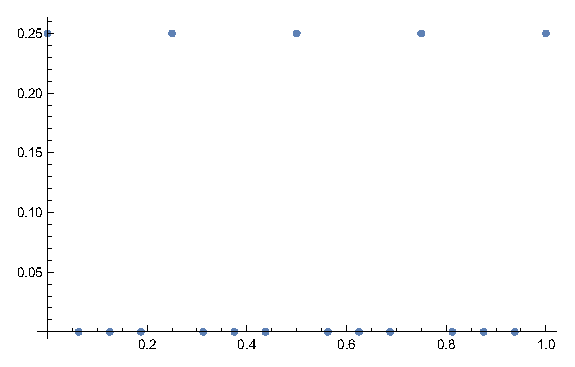
\includegraphics{img/Shor_gr1.eps}

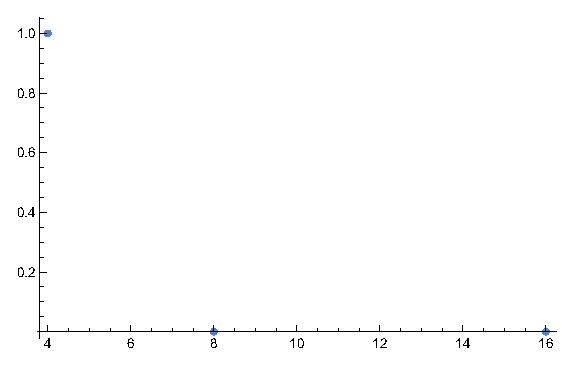
\includegraphics{img/Shor_gr2.eps}

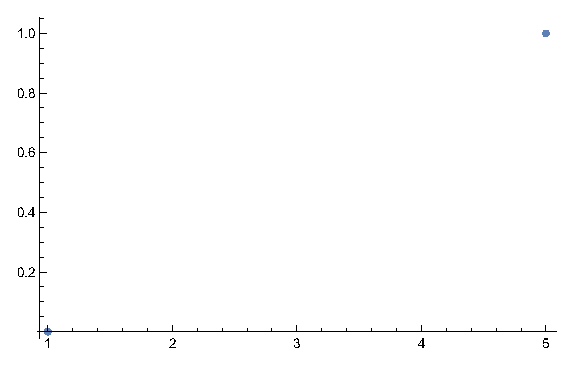
\includegraphics{img/Shor_gr3.eps}

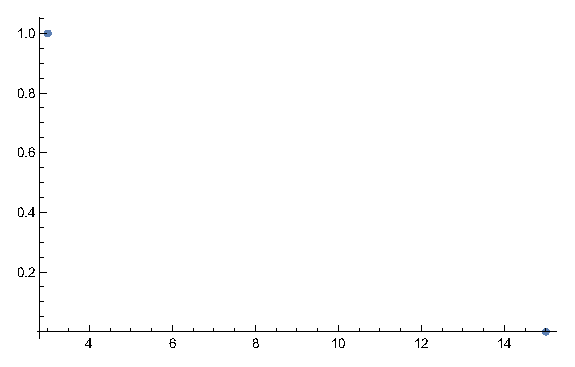
\includegraphics{img/Shor_gr4.eps}

\section{Simulación en Python}

\begin{figure}[H]
\centering 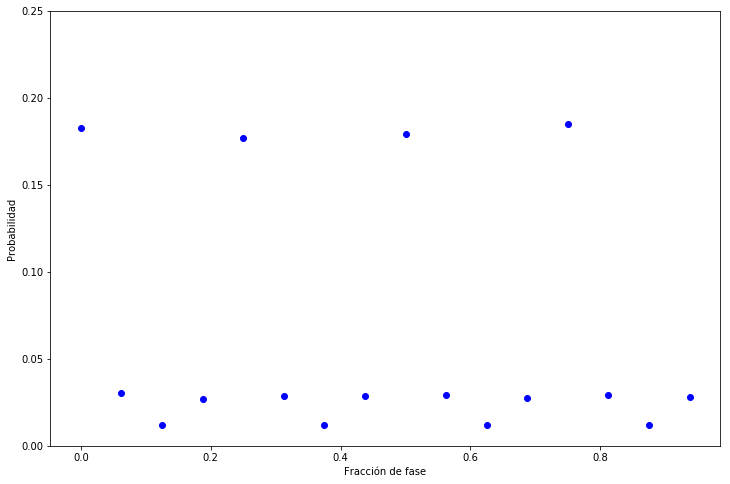
\includegraphics[width=0.9\linewidth]{img/shorlossless.png}
\caption{}
\end{figure}

[0.18265120316248348,
 0.030148605498127055,
 0.0117556126084082,
 0.027068348030583445,
 0.17700021614033762,
 0.028491802773181096,
 0.011881438650927171,
 0.028510782606300467,
 0.17917422966710292,
 0.029450553218688075,
 0.012081135256705483,
 0.027710388875941253,
 0.18489803932544116,
 0.02936951642045106,
 0.012035158723792341,
 0.027772969041529337]

Se ha realizado una simulación del algoritmo de Grover en Wolfram Mathematica implementando $U_{\omega}$, $U_s$ y la transformada de Hadamard, directamente, de manera matricial, de acuerdo a las definiciones dadas anteriormente. Por otro lado, se ha realizado una simulación del algoritmo de Grover en Python definiendo todas las operaciones y transformaciones en base a sus construcciones circuitales, a partir de las compuertas nativas de los transmones, resolviendo la ecuación maestra del sistema al aplicar cada compuerta nativa. A la primera la llamaremos la simulación matemática, y a la segunda, simulación circuital. El código de ambas simulaciones se encuentra en el apédice (APENDICE).

En el caso de la simulación matemática, sólo se ha simulado el caso sin pérdidas. Sin embargo, en el caso de la simulación circuital, se ha simulado el sistema tanto sin pérdidas, como con pérdidas. En el caso del sistema con pérdidas, se ha utilizado la ecuación maestra de Lindblad con los operadores de colapso $\sigma_{-_i}$ y tasa de relajación $\gamma = 25KHz$. Primero compararemos las dos simulaciones sin pérdidas para analizar la precisión del solucionador de ecuaciones maestras.

En la figura (FIGURA) se puede observar la gráfica de la evolución de la probabilidad de medir cada estado en cada iteración. Como se puede observar, ambas figuras son bastante similares. Por otro lado, la fidelidad entre los estados finales de ambas simulaciones es <++>. Por lo que la precisión del solucionador de ecuaciones maestras causó un error correspondiente a una pérdida de <++> de fidelidad.

\begin{figure}[H]
    \centering
    \begin{subfigure}[m]{0.45\textwidth}
        \centering
        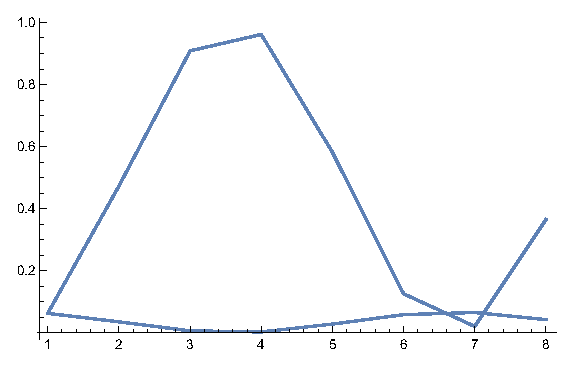
\includegraphics{img/Grover-2_gr1.eps}
        \caption{Rx}
    \end{subfigure}
    \begin{subfigure}[m]{0.45\textwidth}
        \centering
        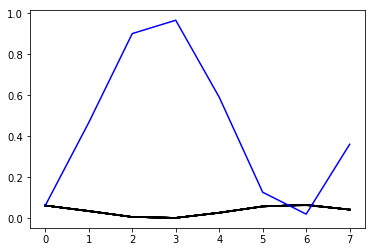
\includegraphics[width=0.9\linewidth]{img/groveralllossless.png}
        \caption{Ry}
    \end{subfigure}
    \caption[]{Compuertas Rx, Ry y Rz en la esfera de Bloch}
    \label{fig:groverlosslesscomp}
\end{figure}

Ahora, compararemos los resultados de la simulación circuital con y sin pérdidas. Como se puede ver en la figura (FIGURA), en el caso con pérdidas, los estados que no contienen el valor deseado dejan de tener la misma probabilidad. Los estados que involucran el estado base ganan probabilidad debido a la relajación de los qubits. La fidelidad entre los estados resultantes de los casos con y sin pérdidas es de <++>.

Aunque la fidelidad sea tan baja, la probabilidad del estado deseado sigue siendo lo suficientemente alta como para obtener el resultado deseado x/x veces.

\begin{figure}[H]
    \centering
    \begin{subfigure}[m]{0.45\textwidth}
        \centering
        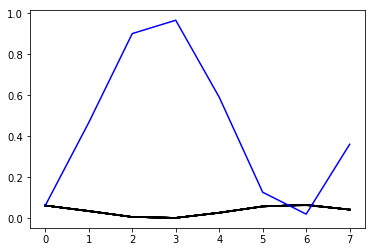
\includegraphics[width=0.9\linewidth]{img/groveralllossless.png}
        \caption{Ry}
    \end{subfigure}
    \begin{subfigure}[m]{0.45\textwidth}
        \centering
        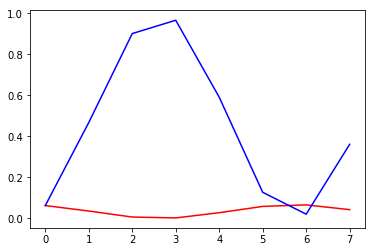
\includegraphics[width=0.9\linewidth]{img/groverpairlossless.png}
        \caption{Rz}
    \end{subfigure}
    \caption[]{Compuertas Rx, Ry y Rz en la esfera de Bloch}
    \label{fig:groverlosscomp}
\end{figure}

